\documentclass[12pt,a4paper,pdflatex]{article}

\usepackage{amsmath}                                       % S\'imbolos matem\'aticos
\usepackage{amsthm}                                        % S\'imbolos matem\'aticos
\usepackage{amssymb}                                       % S\'imbolos matem\'aticos
\usepackage[round, longnamesfirst]{natbib}                 % Referencias bibliogr\'aficas

\usepackage{fancyhdr}                                      % Permite el uso de encabezados
\usepackage{lscape}                                        % Rotacion de la pagina

\usepackage{graphicx}                                      % Insertar figuras
\usepackage{epstopdf}
\usepackage{colortbl}                                      % Trabajar con colores
%\usepackage{hyperref}                                     % V\'inculos y personalizaci\'on del pdf
\usepackage{setspace}                                      % Espacios

\usepackage{rotating}                                      % Tablas horizontales \begin{sidewaystable}
\usepackage{enumitem}                                      % Listas personalizadas
\usepackage{booktabs}                                      % Comandos para tablas, e.g. \toprule
\usepackage{multirow}                                      % Para Tablas. Celdas formadas por m�ltiples filas
\usepackage{tabularx}

\usepackage[spanish]{babel}																 % Idioma espa�ol
\usepackage{float}
\usepackage[centerlast]{subfigure}
\usepackage{rotfloat}
\usepackage{caption}
\usepackage[section]{placeins}
\usepackage{bbm}
\usepackage{anysize}
\usepackage[T1]{fontenc}
\usepackage[utf8]{inputenc}                                %Division del documento
\usepackage{titlesec}
\usepackage[scaled]{uarial}
\renewcommand*\familydefault{\sfdefault}

%Margenes del documento segun formato PUCP
\usepackage[top=4cm,bottom=2.5cm,left=3.5cm,right=2.5cm]{geometry}

%Personalizacion del pdf
\usepackage{color}
\definecolor{darkred}{rgb}{0.5,0,0}
\definecolor{darkblue}{rgb}{0,0,0.5}
\usepackage[colorlinks,breaklinks,bookmarksnumbered,bookmarksopenlevel=2,unicode]{hyperref}               % V\'inculos y personalizaci\'on del pdf
\hypersetup{
  colorlinks,
  citecolor=darkred,
  linkcolor=darkred,
  urlcolor=darkblue,
	bookmarksopen=true, bookmarksopenlevel=3
	}


%%%%%%%%%%%%%%%%%%%% Formato del titulo
\titleformat{\section}[block]
{\normalfont\LARGE\filcenter}{\thesection}{1em}{}



%%%%%%%%%%%%%%%%%%%% Primera p\'agina del art\'iculo (macro \portada)
\def\portada{
\mbox{}\\[-2cm]
\begin{center}
    \mbox{}\\[6mm]
    \large\textsc{\textbf{\institucion}} \\[1mm]
    \large\textsc{\textbf{\facultad}}\\[12mm]
    
\includegraphics[scale=0.5]{logopucp.png}\\[10mm]
    \large\textsc{\textbf{\title}}\\[8mm]
    \large{\textbf{\presentacion}}\\[10mm]
    \large{\textbf{\textoa}}\\[1.75mm]
    \large{\textsf{\author}}\\[8mm]
    \large{\textbf{\textob}}\\[1.75mm]
    \large{\textsf{\asesor}}\\[11mm]
    \large{\textsf{\date}}\\
    %\vspace{15pt}
\end{center}
}


%%%%%%%%%%%%%%%%%%%%%%% Portada

\def\institucion{PONTIFICIA UNIVERSIDAD CAT\'OLICA DEL PERU}
\def\facultad{FACULTAD DE CIENCIAS SOCIALES}
\def\title{El traspaso del tipo de cambio hacia los precios de internet}
\def\presentacion{TESIS PARA OPTAR EL T\'ITULO PROFESIONAL DE LICENCIADO EN ECONOM\'IA}
\def\textoa{AUTOR}
\def\author{Alexandra Carolina Marcos Quispe}
\def\textob{ASESOR}
\def\asesor{Marco Antonio Vega De la Cruz}
\def\date{Agosto, 2020}

%%% Encabezados y pie de p\'aginas and footers eliminate widows and orphan lines
\clubpenalty=100000000
\widowpenalty=10000000

%Doble espacio segun formato pucp
\renewcommand{\baselinestretch}{2}

\begin{document}

%Portada
%%%%%%%%%%
\portada

\thispagestyle{empty}


%Abstract
%%%%%%%%%%
\begin{abstract}
Insertar abstract
\\
Palabras Claves:\\
Clasificaci\'on JEL:
\end{abstract}
\thispagestyle{empty}
\clearpage

%%% Contenido
\tableofcontents
\thispagestyle{empty}
\clearpage
\listoffigures
\thispagestyle{empty}
\clearpage
\listoftables
\thispagestyle{empty}
\clearpage

\pagenumbering{roman}
\newpage
%-----------------------------------------------Nuevo capitulo-----------------------------------------
\section{Introducci\'on}\label{sec1}

En la actualidad, los pa\'ises se encuentran ante una revoluci\'on digital que proyecta el incremento de miles de millones de conexiones entre personas, procesos industriales y de negocios, y de datos. Este proceso tiene por denominaci\'on el internet de las cosas (Internet of Everything) y se estima que generar\'a enormes oportunidades de progreso para los pa\'ises \citep{lombardero2015trabajar}.

La digitalizaci\'on de la econom\'ia est\'a estrechamente ligado con esta transformaci\'on tecnolog\'ica, basado en la convergencia de redes y aplicaciones que permitir\'a garantizar la sostenibilidad econ\'omica y social \citep{lombardero2015trabajar}. Dentro del crecimiento de nuevos procesos, el m\'as relevante es la distribuci\'on comercial del sector retail.

El mercado retail se caracteriza por el comercio de ventas al por menor. Dentro de este sector se encuentran las tiendas por departamento, los centros comerciales, las tiendas de conveniencia, entre otras. La creaci\'on de un nuevo canal de distribuci\'on comercial ha cambiado la forma en c\'omo se relacionan los consumidores, las firmas o tiendas retail e incluso los trabajadores \citep{rey2017transformacion}. 

El espectacular crecimiento de la distribuci\'on comercial a trav\'es del canal online, y en particular la venta v\'ia dispositivos m\'oviles, es signo claro de esta transformaci\'on. Esta nueva forma de comercializaci\'on virtual del mercado retail se le denomina "`e-commerce"' y su creaci\'on genera, actualmente, la mayor\'ia del crecimiento de ventas de mucho de estas tiendas \citep{global2016global}.

La transformaci\'on digital de las tiendas f\'isicas hacia tiendas m\'as omnipresentes ha dado paso a la creaci\'on de nuevas variables econ\'omicas como son los precios de internet. La recolecci\'on de esta informaci\'on contenida en las paginas web de las tiendas retail ha sido posible gracias al avance digital de los datos. La creaci\'on de programas automatizados como el "`scraping"' permiten, a costo bajo, la implementaci\'on y el dise\~no de larga escala de recolecci\'on de datos en la web \citep{cavallo2016billion}.

Inicialmente, el uso de estos nuevos datos recolectados de las paginas web eran utilizados en investigaciones que buscaban caracterizar el comportamiento de los precios a nivel microecon\'omico \citep{cavallo2018scraped}. Asi como, encontrar diferencias o similaridades con los precios tradicionales. Sin embargo, el avance de este sector ha dado paso a un nuevo tipo de investigaciones que buscan entender la vulnerabilidad de los precios de internet ante los choque macroecon\'omicos.

En el Per\'u, el comercio electr\'onico ha sido ampliamente aceptado y ello, se refleja en el aumento de las tasas de crecimiento de sus ventas y sus proyecciones de ventas.

Por otro lado, la vulnerabilidad de las econom\'ias abiertas y dolarizadas como la peruana tiene en parte su origen en las fluctuaciones del tipo de cambio. La literatura tradicional concluye que el efecto traspaso del tipo de cambio ha ido disminuyendo hasta tener una magnitud muy reducida, lo que ha ido restando su importancia. Sin embargo, la aparici\'on de un nuevo tipo de precio, el precio de internet, ha despertado el inter\'es por estudiar su grado de reacci\'on ante los movimientos cambiarios y otros choques macroecon\'omicos.

El presente trabajo se centra en estudiar el grado de reacci\'on de los precios de internet ante fluctuaciones cambiarias utilizando un enfoque microecon\'omico para el sector retail en el Per\'u. Esto se basa en la reciente literatura que busca explicar traspaso incompleto y reducido hacia los precios de los consumidores usando un enfoque microecon\'omico.

\textcolor[rgb]{1,0.41,0.13}{Explica literatura de esto}

\textcolor[rgb]{1,0.41,0.13}{PREGUNTA DE INVESTIGACION:
}A la luz de lo expuesto, se busca responder la siguiente pregunta de investigaci\'on: 


\textcolor[rgb]{1,0.41,0.13}{RESUMEN DE LA ESTRUCTURA DEL DOCUMENTO
} 
\newpage
%-----------------------------------------------Nuevo capitulo-----------------------------------------
\section{Marco Te\'orico}\label{sec2}

En una econom\'ia abierta, los precios dom\'esticos de los bienes transables, importados o finales denominados en moneda extranjera est\'an expuestos a choques macroecon\'omicos como son los incrementos o disminuciones del tipo de cambio. El efecto de las fluctuaciones cambiarias sobre el nivel de precios, sin precisar exactamente los canales de transmisi\'on, se le denomina \textit{el traspaso del tipo de cambio} \citep{winkelried2003}. 

En otras palabras, el traspaso del tipo de cambio busca cuantificar el grado de reacci\'on de los distintos precios ante variaciones del tipo de cambio para una determinada econom\'ia. Ello, le permite a los Bancos Centrales tener un mecanismo de pol\'itica monetaria que le posibilite disminuir la vulnerabilidad de los choques externos, no solo sobre el precios sino tambi\'en sobre el producto.

Existen tres tipos de precios donde cada uno representan un nivel en la cadena distributiva de bienes. En el primer nivel, se determinan los precios de los bienes importados que se destinan al consumo directo, tambi\'en denominados precios de importaci\'on al por mayor. En el siguiente nivel, se determinan los precios al por mayor o precios de los productores y en el \'ultimo, los precios al por menor o precio de los consumidores \citep{miller2003}.

El grado de reacci\'on de los precios en cada nivel depender\'a de la disposici\'on de sacrificar m\'argenes de ganancia. El efecto de una depreciaci\'on del tipo de cambio afecta directamente a los precios de las importaciones, este efecto puede ser asumido completamente y no alterar sus precios lo que implicar\'ia una disminuci\'on en sus m\'argenes de ganancia. Caso contrario, la firma puede aumentar sus precios y todo el efecto de la subida ser\'a asumido por lo consumidores.

Esta interrelaci\'on \textit{directa} de precios permite entender la din\'amica de un choque cambiario y, adicionalmente, incorporar otros canales de an\'alisis como el microecon\'omico. En particular, en \citet{burstein2014international} se modela esta interrelaci\'on de los precios de los consumidores y los precios de las importaciones. Las variaciones del precio del consumidor est\'an explicados por tres componentes, los cambios en los precios de los servicios de distribuci\'on, las variaciones del margen de la tienda minorista y los cambios del precio de las importaciones. El primer componente se refiere a los costos que asume la tienda minorista al ofrecer sus servicios locales como costo del local o la mano de obra. El impacto de una depreciaci\'on cambiaria sobre los precios minoristas se explicar\'ia por dos de estos canales: el aumento del precio de las importaciones y la disminuci\'on del margen.

Adicionalmente, existe una interrelaci\'on \textit{indirecta} donde las firmas productoras cuyos precios se denominan en moneda local se ven afectados a trav\'es de un incremento de los costos de los insumos que se denominan en moneda extranjera. Tal como la relaci\'on anterior, la firma decidir\'a si sacrificar o no margen y traspasarlo hacia los consumidores \citep{winkelried2012traspaso}.

Existe una amplia metodolog\'ia de estudios del traspaso que dependen del tipo de datos a utilizar (datos agregagos o desagregados) y de los problemas que cada uno de las bases conlleva. Pese a ello, es posible caracterizar cuatro aspectos importantes: la magnitud del traspaso, la velocidad de ajuste, la simetr\'ia y la no linealidad.

La ecuaci\'on \ref{eq1} simplifica la relaci\'on del tipo de cambio y los precios. Donde $P_{t}$ es el precio en el periodo $t$ y $S_{t}$ es tipo de cambio nominal en el periodo $t$. 

\begin{equation} \label{eq1}
  \Delta P_{t} = \alpha_{0} +\alpha_{1}P_{t-1} +\alpha_{2}\Delta S_{t}
\end{equation}

Asumiendo que un choque cambiario ex\'ogeno impacta sobre los precios, la ecuaci\'on anterior se puede expresar de la siguiente forma.
\begin{equation}\label{eq2}
  \Delta P_{t} = \alpha_{0} +\alpha_{1}P_{t-1} +\alpha_{2}\delta
\end{equation}

La magnitud del coeficiente del traspaso, mide la proporci\'on del cambio en el tipo de cambio que se va a trasladar a los precios. En la ecuaci\'on \ref{eq2} se observa que un incremento en $\delta$ porciento, la magnitud de traspaso est\'a representada por el coeficiente $\alpha_{2}$. Este coeficiente puede tomar valores entre $0$ y $1$, y se afirma que el traspaso es incompleto hacia las precios cuando el coeficiente es menor a la unidad. Ello, indica que el trapaso es menor que proporcional al cambio en el tipo de cambio. Por el contrario, se dice que el traspaso es completo cuando es exactamente igual a la variaci\'on del tipo de cambio. Es decir, el coeficiente $\alpha_{2}$ toma 

Asimismo, el impacto se puede diferenciar por el tiempo de reacci\'on de los precios como consecuencia del choque. La reacci\'on inmediata al cambio del tipo de cambio se le denomina traspaso de \textit{corto plazo} y la magnitud final cuando el precio alcanza su nuevo equilibrio, luego del choque, se le denomina traspaso de \textit{largo plazo}.

El coeficiente $\alpha_{2}$ representa el traspaso de corto plazo dado que mide la proporci\'on de reacci\'on de los precios en el mismo periodo $t$ que ocurre el choque. 

Reescribiendo la ecuaci\'on \ref{eq2}, se puede despejar el precio en funci\'on del precio del periodo previo y el choque.
 $$P_{t}- P_{t-1} = \alpha_{0} +\alpha_{1}P_{t-1} +\alpha_{2}\delta$$
\begin{equation} \label{eq4}
 P_{t} = \alpha_{0} + (1+\alpha_{1})P_{t-1} + \alpha_{2}\delta \\
 \end{equation}

Donde $\alpha_{1}<0$ y un aumento del tipo de cambio en $\delta \%$ son par\'ametros que determinan el nuevo precio de equilibrio $\overline{P}$. Este se muestra en en la ecuaci\'on \ref{eq5}:

\begin{equation} \label{eq5}
 \overline{P} =  \alpha_{0} + (1+\alpha_{1})\overline{P}+ \alpha_{2}\delta
\end{equation}

$$\overline{P} = \frac{-1}{\alpha_{1}}(\alpha_{0}+\alpha_{2}\delta)$$

La ecuaci\'on \ref{eq6} muestra el precio de equilibrio $\overline{P'}$ previo al choque. La diferencia del nuevo precio de equilibrio luego del choque y el precio de equilibrio previo al choque muestra el coeficiente de magnitud de largo plazo. Este se define como la proporci\'on de reacci\'on total de los precios.
\begin{equation} \label{eq6}
 \overline{P'} = \alpha_{0} + (1+\alpha_{1})\overline{P'}
\end{equation}
$$\overline{P'} = \frac{-\alpha_{0}}{\alpha_{1}}$$

El traspaso de largo plazo, se escribe de la siguiente forma:
\begin{equation} \label{eq7}
 \overline{P} = \overline{P'} - \frac{\alpha_{2}}{\alpha_{1}}\delta
\end{equation}
$$\overline{P} - \overline{P'} = -\textcolor[rgb]{1,0,0}{\frac{\alpha_{2}}{\alpha_{1}}}\delta$$
Donde un incremento de $\delta$ por ciento resulta en un coeficiente de traspaso de largo plazo de $\frac{\alpha_{2}}{\alpha_{1}}$ por ciento.
Asimismo, la proporci\'on del cambio del tipo de cambio hacia los precios puede tomar valores desde 0 hasta 1. De la misma manera, si los precios reaccionan en la misma magnitud a la variaci\'on del tipo de cambio, el traspaso se le denomina completo. Por el contrario, si los precios reaccionan en una menor proporci\'on se le denomina traspaso incompleto.

Seguidamente, el tiempo que demore el precio $\overline{P'}$ en alcanzar su estado de equilibrio $\overline{P}$ luego del choque se le denomina \textit{la velocidad de ajuste}. Los precios pueden responder en el momento $t$ de manera inmediata al choque y por lo tanto, tener una magnitud de traspaso completo. O caso contrario, gradualmente alcanza su nuevo precio de equilibrio en $t + k$ periodos.

La ecuaci\'on \ref{eq1} presenta una versi\'on simplicada de la relaci\'on del tipo de cambio con los precios donde la magnitud de respuesta es igual ante una depreciaci\'on o una apreciaci\'on del tipo de cambio.
Sin embargo, la evidencia emp\'irica demuestra que tanto la magnitud como la velocidad de ajuste del traspaso es diferente en cada situaci\'on. Esta diferencia se denomina la asimetr\'ia del traspaso donde un aumento de $\delta \%$ del tipo de cambio (depreciaci\'on) es diferente el impacto a una disminuci\'on (apreciaci\'on).
Incorporando las asimetr\'ias en la ecuaci\'on \ref{eq1}, se reemplaza $\alpha_{2}\Delta S_{t}$ por:
\begin{equation}
  \Delta P_{t} = \alpha_{0} +\alpha_{1}P_{t-1} +\alpha_{2A}A\Delta S_{t} + \alpha_{2D}D\Delta S_{t}
\end{equation}
Donde $A$ y $D$ se activan cuando se aprecia o se deprecia el tipo de cambio respectivamente. La literatura explican que las asimetr\'ias se explican ante una mayor rigidez hacia bajo comparado con la rigidez hacia arriba.

Finalmente, la no linealidad estudia el impacto diferenciado de peque�o movimiento del tipo de cambio contra un movimiento brusco. Este fen\'omeno implicaba que el comportamiento de los precios eran distinto ante subidas disruptivas en comparaci\'on de un incremento moderado del tipo de cambio.
\begin{equation} \label{eq7}
  \Delta P_{t} = \alpha_{0} +\alpha_{1}P_{t-1} +\alpha_{2H}H\Delta S_{t} + \alpha_{2S}S\Delta S_{t}
\end{equation}
Donde $H$ se activa cuando ocurre un cambio del tipo de cambio superior a un umbral $\overline{\delta}$ y contrario, $L$ se activa cuando ocurre un cambio del tipo de cambio inferior al umbral $\overline{\delta}$. Esta ecuaci\'on un incremento del tipo de cambio fuerte, en el corto plazo, esta capturado por el coeficiente $\alpha_{2H}$ y ante un incremento moderado, la magnitud de traspaso est\'a capturado por $\alpha_{2S}$.

Adicionalmente, existe otra metodolog\'ia que permite cuantificar el traspaso del tipo de cambio condicionado al cambio de precios. Este captura el efecto del traspaso en una base restringida que no incorpora las observaciones que no presentan cambios de precios. De esta manera se puede obtener el traspaso de mediano plazo ("`Medium-run pass-through"') y el traspaso de larga vida ("`Life-long pass-through"').

El traspaso de mediano plazo cuantifica el efecto acumulado del movimiento del tipo de cambio a lo largo de la duraci�n de la vigencia del precio anterior y el traspaso de larga vida implica acumular los cambios de precios y los cambios en el tipo de cambio a lo largo de toda la vida del bien en la muestra \citep{burstein2014international}. Esta \'ultima metodolog\'ia ser\'a presentada a mayor detalle en el cap\'itulo cuatro.


\newpage
%-----------------------------------------------Nuevo capitulo-----------------------------------------
\section{Revisi\'on de la literatura}\label{sec3}

Los estudios cl\'asicos del traspaso de tipo de cambio cuantifican la magnitud de respuesta de los precios ante fluctuaciones cambiarias, utilizando informaci\'on a nivel agregada. Los resultados de estas investigaciones indican que existe un nivel de traspaso incompleto de corto y largo plazo para los diferentes \'indices de precios en la literatura \citep{burstein2014international, bussiere2013exchange}.

Los hallazgos emp\'iricos muestran que el \'indice de precios al consumidor (IPC) presenta una sensibilidad uniformemente menor comparado con el \'indice de precios a las importaciones (IPI).
Dentro de una muestra de nueve econom\'ias desarrolladas\footnote{Estados Unidos, Jap\'on, Italia, Reino Unido, Francia, Alemania, Canad\'a y Suiza}, se resalta el caso de Estados Unidos. Su coeficiente de traspaso de corto y largo plazo para el \'indice de precios a las importaciones ($20\%$ y $51\%$) es por lo menos el doble comparado con el \'indice de precios al consumidor ($6\%$ y $17\%$) \citep{burstein2014international}.

A partir de ello, se evidencia el bajo grado de reacci\'on de los precios al consumidor en comparaci\'on del resto de indicadores y esto se refleja en una baja variac\'ion de los precios de la tiendas de menor comercio.
Este fen\'omeno se demuestra en \citet{mccarthy2007} donde ocurre una disminuci\'on del traspaso sobre el CPI para las nueve econom\'ias de la OECD. De acuerdo a las estimaciones, el traspaso ha ido disminuido por lo menos en un $50\%$ desde el a\~no 1983.

Asimismo, el bajo grado de reacci\'on de los precios ante choques cambiarios se ha presentado en las econom\'ias latinoamericanas. En el caso peruano, el \'indice de precios a las importaciones (IIP) presenta un coeficiente del $85\%$ y el \'indice de precios al consumidor (IPC) un $46\%$ de respuesta. La conclusi\'on para el Per\'u es un traspaso peque\~no que ha ido disminuyendo en los \'ultimos a\~nos \citep{winkelried2003}, sobretodo esta rigidez es m\'as visible para el CPI.

En este contexto econ\'omico, se han presentado distintos factores que expliquen el bajo grado de reacci\'on de los precios. Un factor resaltante es la adopci\'on de esquemas de metas de inflaci\'on y el nuevo r\'egimen cambiario denominado flotaci\'on sucia que ha originado una mayor estabilidad de los precios \citep{winkelried2003}. 

Por otro lado, esta disminuci\'on del nivel de traspaso puede explicarse conjuntamente a trav\'es de factores microecon\'omicos.

En \citet{taylor2000} se plantea que detr\'as del bajo nivel de traspaso sobre los precios y los costos en Estados Unidos est\'a explicado por la ca\'ida del poder de fijaci\'on de precios por parte de las empresas. A trav\'es de un modelo microecon\'omico, se evidencia que los cambios observados en el poder de fija precios se deben, en parte, a cambios en las expectativas de los movimientos de alterar precios y costos. Exactamente, una firma estar\'ia dispuesta a subir sus precios o costos, si espera que los cambios realizados sean permanentes.

En vista del surgimiento de estudios microfundados, la literatura actual del traspaso busca examinar los factores que est\'an detr\'as de este coeficiente incompleto, a trav\'es del uso de datos desagregados. De los cuales, var\'ian dependiendo del or\'igen de recolecci\'on. El primer grupo de datos se obtiene del conjunto de informaci\'on desagregada del IPC, tambi\'en est\'an aquellos datos que se recolectan escaneando directamente el precio del producto de las tiendas. El segundo grupo de datos, y los m\'as utilizados en la actualidad, son los datos \textit{escrapeados} cuyo bajo costo y facilidad de obtenci\'on radica en el hecho que es informaci\'on recolectada directamente de las p\'aginas de internet de las tiendas minoristas.

Este \'ultimo grupo de datos ha dado surgimiento a una nueva variable econ\'omica conocida como los precios de internet. Una gran variedad de tiendas minoristas ofrecen sus productos a trav\'es de dos canales de ventas, su canal f\'isico en donde se realizan las transacciones en la propia tienda y el canal virtual, donde se realizan las transacciones utilizando la p\'agina web.

Esta novedosa forma de recolecci\'on de informaci\'on ha permitido, a la par, continuar con las investigaciones que estudian el bajo grado de traspaso a un nivel muy espec\'ifico. Al mismo tiempo, enfocarse en analizar el grado de reacci\'on de una nueva variable como es el precio de internet \citep{cavallo2016}. Tal nivel de desagregaci\'on ha permitido la identificaci\'on \'unica de los productos y por consiguiente, la obtenci\'on de caracter\'isticas espec\'ificas del bien como son la locaci\'on de la tienda, el grado de competencia a nivel de locaci\'on, la finalidad de uso del bien, si son productos importados o producidos localmente e incluso a nivel de caracter\'isticas del precio como su frecuencia de ajuste y la duraci\'on. \citep{NBERw20406,Gopinath2010,kim2003,gopinath2010itskhoki}.

Es clave resaltar que a este nivel de desagregaci\'on cambia la perspectiva de un traspaso \'unico para toda la base de datos y se utiliza el t\'ermino traspaso heterog\'eneo que depender\'a de las caracter\'isticas a nivel de producto. En ese sentido, se realiza un resumen de las principales variables microecon\'omicas que explican el comportamiento poco flexible de los precios.

\subsection{El poder de mercado y el grado de competencia}
La literatura encuentra que el traspaso incompleto del tipo de cambio hacia los precios estar\'a asociado con el poder de mercado.  
En particular, en \citet{feenstra1996} se estudia el comportamiento de los precios de los productos importados a nivel del agente exportador y el grado reacci\'on cambiaria en el mercado de autos importados en Estados Unidos.

Se estima que las firmas en los pa\'ises exportadores con una participaci\'on de mercado muy alta, cercana al 100\%, tendr\'an un traspaso alto sobre los precios. Sin embargo, debajo del umbral del 40\% de participaci\'on la relaci\'on no es completamente lineal y depender\'a de otros factores tales como el comportamiento de la demanda y las interacciones con las otras firmas.

En este caso es posible hablar de participaci\'on de mercado como variable que cuantifique el poder de mercado de cada firma tal como lo define la literatura. No obstante, en otros estudios desagregados la informaci\'on individual de las ventas de las tiendas es problem\'atico de obtener. En ese sentido, en \citet{NBERw20406} se utiliza como variable proxy de la participaci\'on de mercado el n\'umero de vendedores que afronta la tienda minorista. Los resultados reafirman lo estimado en \citet{feenstra1996}, se encuentra una relaci\'on no lineal entre el trapaso y el n\'umero de vendedores. El traspaso es creciente en el n\'umero de tiendas cuando el rango de firmas est\'e entre 2 y el promedio de la muestra, 5. En cambio el traspaso es decreciente cuando se sobrepasa el umbral de 5 tiendas competidoras.

As\'i como el n\'umero de vendedores cuantifica la participaci\'on de mercado esta variable tambi\'en captura el grado de competencia. Al respecto, en \citet{castellares2017} se estima el traspaso del tipo de cambio sobre el mercado de autos usados en el Per\'u. Para ello, utilizan la informaci\'on de los anuncios de autos usados publicados en los avisos del diario El Comercio e incorporan la variable estrechez del mercado cuantificando del n\'umero de d\'ias que demora un auto en ser vendido. 

Conforme con los resultados, un traspaso del tipo de cambio es menor cuando la estrechez del mercado aumenta o existe un mayor nivel de competencia. Este resultado difiere con lo encontrado en la literatura cl\'asica; sin embargo, lo particular de esta investigaci\'on es el estudio de un mercado muy espec\'ifico utilizando datos desagregados.

Por el contrario, es consistente con lo encontrado en \citet{kim2003} en el mercado del trigo donde se evidencia que en Jap\'on, pa\'is con mayor competencia se estima un traspaso bajo. En cambio, en Corea donde existe un mercado oligop\'olico se estima un traspaso mayor. \colorbox[rgb]{0.92,0.5,0.4}{FALTA EXPLICAR los canales}

\subsection{El nivel de calidad del producto}
Adicionalmente, otro factor relacionado con el bajo grado de reacci\'on cambiaria de los precios es la calidad del producto. Con la finalidad de capturar esta variable, algunas investigaciones comparan el precio hist\'orico del bien con la mediana de los precios hist\'oricos totales. Con esta informaci\'on se puede identificar dos bloques de productos, productos caros o baratos, y analizar el comportamiento del traspaso en estos.

En \citet{castellares2017} tambi\'en se incorporar esta variable dicot\'omica que toma los valores de $1$ o $0$ y se clasifica si el bien es de calidad alta o calidad baja respectivamente. Los resultados muestran que el traspaso del tipo de cambio a los precios en soles en los
autos de mayor calidad es 35.5 \% m\'as bajo que en los autos de menor calidad. Este resultado es consistente con las predicciones en \citet{auer2009exchange}, donde el traspaso del tipo de cambio es menor en bienes de mayor calidad.
Esta relaci\'on se vuelve m\'as interesante cuando se realizan estudios con precios de bienes de tiendas minoristas, debido a que se incorporan un rango de bienes mucho menor comparado con los precios de autom\'oviles de las anteriores investigaciones. En \citet{NBERw20406} se estima que existe un traspaso en forma de U invertida, para bienes que est\'an por debajo del precio mediano de $\$150$ d\'olares se presenta una relaci\'on negativa donde a mayor tama\~no del precio menor ser\'a el traspaso. Por otro lado, en bienes por encima de los $\$150$d\'olares se presentaba la relaci\'on negativa, a mayor tama\~no del precio menor ser\'a el traspaso, consistente con las relaciones mencionadas.

La relaci\'on U invertida del traspaso con la calidad del producto se relaciona a trav\'es de los costos de busqueda \citep{NBERw20406}. Los bienes categorizados como calidad alta son aquellos que tienen un precio por encima del promedio. Ello implica que al ser bienes costosos incentivan a los compradores a comparar precios entre tiendas previo a una decisi\'on de compra. Es decir, son bienes intensivos en b\'usqueda cuya acci\'on genera un alto retorno al comprador. Esta acci\'on de comparar precios genera una presi\'on sobre las tiendas y firmas lo que a su vez determina una juego simult\'aneo entre esta dos variables, precio y nivel de busqueda. La respuesta de las firmas es fijar un nivel de precios que determine cierto nivel de b\'usqueda y a consecuencia, los retornos de b\'usqueda para los bienes costosos sean bajos \citep{NBERw20406}. 

\subsection{La categor\'ia del producto: finalidad de uso}
La categor\'ia del bien ha sido una variable poco implementada en el an\'alisis de la heterogeneidad del traspaso pero si utilizada en estudios que analicen el comportamiento de los precios a partir de esta clasificaci\'on. En \citet{nakamura2013price}

\subsection{Frecuencia de ajuste de precios}
\subsection{Inventario}
\colorbox[rgb]{0.92,0.5,0.4}{poner las categorias, frecuencia, inventario y resumen.}

\newpage

%-----------------------------------------------Nuevo capitulo-----------------------------------------
\section{Metodolog\'ia}\label{sec4}
La finalidad de la presente investigaci\'on es estimar el traspaso del tipo de cambio hacia esta nueva variable econ\'omica, denominada los precios de internet. Asimismo, la literatura ha demostrado que a nivel agregado el traspaso es incompleto y gradual, aunque la posibilidad de incorporar factores microec\'omicos permite extender el comportamiento de los precios a un nivel de detalle mayor.

En ese sentido, se plantea la metodolog\'ia propuesta en \citet{gopinath2010itskhoki} denominada el \textbf{Traspaso de Larga Vida} (Life-Long PassThrough: LLPT). Esta metodolog\'ia no estructural propone que el nivel del traspaso de los bienes dependa de variables que caractericen el comportamiento de los precios. Ello, a trav\'es del uso de datos desagregados que posibilitan identificar propiedades a nivel de producto.
Este enfoque trabaja \'unicamente con observaciones donde se presenten cambios de precios y estima el traspaso del tipo de cambio acumulado sobre la vida de un precio en la base de datos de estudio.

En la figura ~\ref{fig:1} se muestra un ejemplo hipot\'etico de la trayectoria de un precio y la trayectoria del tipo de cambio nominal, ambos en logaritmos desde el periodo $t = 0$ hasta $t = 40$. En el periodo $t=25$ se produce un incremento del precio del bien $i$ lo que lleva al nacimiento de un nuevo precio hasta su desaparici\'on en el periodo $t=33$. La metodolog\'ia de \citet{gopinath2010itskhoki} estima la variaci\'on acumulada del tipo de cambio durante la duraci\'on. Esto se aplica para el resto de observaciones que desagrega cada movimiento de los precios como \'unicas observaciones con su respectivo variaci\'on acumulada del tipo de cambio.

Sin embargo, esta metodolog\'ia se vuelve inv\'alida al momento de trabajar con precios de tiendas minoristas donde una gran parte de sus productos son importados para el caso peruano. Las tiendas minoristas como Saga Falabella presentan un manejo de inventarios con la finalidad de cumplir con el abastecimiento continuo de sus productos. En ese sentido, las compras realizadas por estas tiendas se exponen al movimiento del tipo de cambio no en el momento del ofrecimiento del producto sino cuando se realiza la transacci\'on de compra con el proveedor extranjero.
Es decir, la exposici\'on al riesgo cambiario se produce semanas antes de que el producto sea ofrecido en la p\'agina web.

Por tal raz\'on, la metodolog\'ia utilizada en esta investigaci\'on incorpora el factor inventario al usado en \citet{gopinath2010itskhoki} y estima la variaci\'on acumulada del tipo de cambio 20 d\'ias hacia atr\'as manteniendo la ventana de duraci\'on del precio. Esta idea se representa en la figura ~\ref{fig:1}, donde ahora la variaci\'on acumulada del tipo de cambio se calcula del periodo $t = 13$ contra $t =5$.

\begin{figure}[h] 
\centering
 \caption{Ilustraci\'on de la metodolog\'ia: Life Long PassThrough}
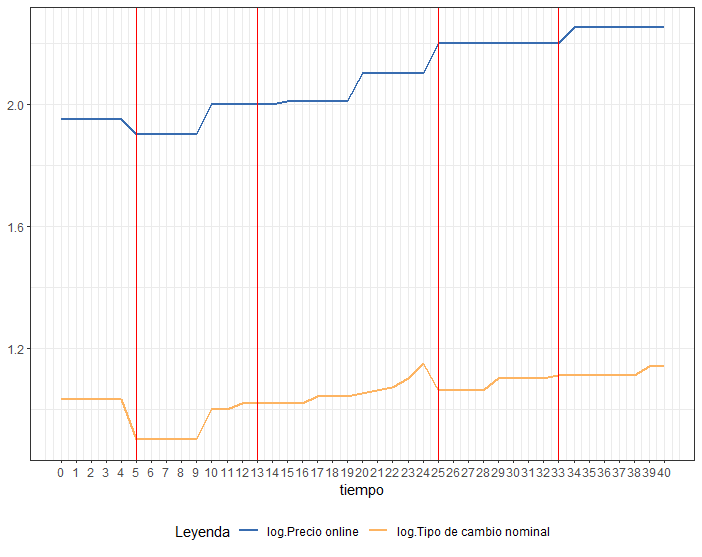
\includegraphics[scale=0.7]{metodologia.png}
  \label{fig:1}
\end{figure}

El traspaso de larga vida se obtiene con la siguiente ecuaci\'on econom\'etrica:
\begin{equation} \label{eq10}
\Delta P_{it} = \beta_{0} +\beta_{1} \Delta S_{it}  + \beta_{2} \Delta S_{it}*X_{i} + \beta_{3}X_{i} + \beta_{4}\psi + \beta_{5}Z + \varepsilon_{it}
\end{equation}

Donde $\Delta P_{it}$ representa el cambio acumulado del precio desde la primera observaci\'on del nuevo precio hasta el nacimiento del siguiente, $\Delta S_{it}$ representa el cambio acumulado del tipo de cambio durante la duraci\'on del respectivo precio, rezagado 20 d\'ias atr\'as.
$X_{i}$ es el factor que captura la heterogenidad del traspaso debido a que incorpora las caracter\'isticas propias de los bienes. En la metodolog\'ia original en \citet{gopinath2010itskhoki} se establece la frecuencia de ajuste de precios como principal variable que explica la heterogeneidad del traspaso. La variable dummy $\psi$ muestra la clasificaci\'on de los productos seg\'un su uso y por �ltimo, $Z$ el grupo de variables control que contiene las variables duraci\'on del precio (d\'ias) y una dummy que controla por ofertas\footnote{Los productos de tiendas minoristas suelen tener d\'ias de descuentos que explica gran parte del movimiento de precios}.

El comercio electr\'onico presenta dias claves donde los precios de los productos presentan una ca\'ida y este efecto no necesariamente se explica por un apreciaci\'on cambiaria sino por dias de descuentos que afectan a todos los precios.

La heterogenidad del traspaso se captura no solo por la inclusi\'on de la caracter\'istica del bien en niveles sino tambi\'en por la variable interactiva que multiplica la variaci\'on del tipo de cambio acumulado por la caracter\'istica del bien.

La primera regresi\'on que se deriva de la metodolog\'ia generaliza es que el traspaso del tipo de cambio depende de la frecuencia de ajuste de precios del bien. Esta relaci\'on esta capturada por la siguiente ecuaci\'on:
\begin{equation}
\Delta P_{it} = \beta_{1} \Delta S_{it}  + \beta_{2} \Delta S_{it}*f_{i} + \beta_{3}f_{i} + \beta_{4}Categorias + \beta_{5}Controles_{i} + \varepsilon_{it}
\end{equation}
Donde $f_{i}$ cuantifica la frecuencia de ajuste de precios de cada bien.

La segunda regresi\'on que se deriva relaciona si un precio denominado caro o barato determina el nivel del traspaso del tipo de cambio y esto se representa en la siguiente ecuaci\'on.
\begin{equation}
\Delta P_{it} = \beta_{1} \Delta S_{it}  + \beta_{2} \Delta S_{it}*P_{i} + \beta_{3}P_{i} + \beta_{4}Categorias + \beta_{5}Controles_{i} + \varepsilon_{it}
\end{equation}
Donde $P_{i}$ es el precio inicial del bien y captura el tama�o del precio.

\clearpage

%-----------------------------------------------Nuevo capitulo-----------------------------------------

%\bibliographystyle{chicago}
\bibliographystyle{chicago}                            % Estilo bibliogr\'afico compatible con natbit, otros no funcionaban :c
\bibliography{TesisBIB}


\end{document} 
